% Created 2017-02-08 Wed 16:29
\documentclass[11pt]{article}
\usepackage[utf8]{inputenc}
\usepackage[T1]{fontenc}
\usepackage{fixltx2e}
\usepackage{graphicx}
\usepackage{longtable}
\usepackage{float}
\usepackage{wrapfig}
\usepackage{rotating}
\usepackage[normalem]{ulem}
\usepackage{amsmath}
\usepackage{textcomp}
\usepackage{marvosym}
\usepackage{wasysym}
\usepackage{amssymb}
\usepackage{hyperref}
\tolerance=1000
\author{David A. Ventimiglia\thanks{dventimi@gmail.com}}
\date{\textit{<2017-02-08>}}
\title{Advanced Lane Lines}
\hypersetup{
  pdfkeywords={},
  pdfsubject={},
  pdfcreator={<a href="http://www.gnu.org/software/emacs/">Emacs</a> 24.5.1 (<a href="http://orgmode.org">Org</a> mode 8.2.10)}}
\begin{document}

\maketitle

\index{Machine-Learning!Self-Driving Cars}
\index{Udacity!Self-Driving Car Nano-Degree Program}

\section*{Introduction}
\label{sec-1}

\section*{Methods}
\label{sec-2}

The goals / steps of this project are the following:

\begin{itemize}
\item Compute the camera calibration matrix and distortion coefficients
given a set of chessboard images.
\item Apply a distortion correction to raw images.
\item Use color transforms, gradients, etc., to create a thresholded
binary image.
\item Apply a perspective transform to rectify binary image ("birds-eye
view").
\item Detect lane pixels and fit to find the lane boundary.
\item Determine the curvature of the lane and vehicle position with
respect to center.
\item Warp the detected lane boundaries back onto the original image.
\item Output visual display of the lane boundaries and numerical
estimation of lane curvature and vehicle position.
\end{itemize}

\subsection*{Setup}
\label{sec-2-1}

\begin{verbatim}
from collections import deque
from itertools import groupby, islice, zip_longest, cycle, filterfalse
from matplotlib.collections import PatchCollection
from matplotlib.patches import Polygon
from matplotlib.widgets import Button
from matplotlib.widgets import Slider, Button, RadioButtons
from moviepy.editor import VideoFileClip
from mpl_toolkits.axes_grid1 import ImageGrid
import cProfile
import cv2
import glob
import matplotlib
import matplotlib.image as mpimg
import matplotlib.pyplot as plt
import numpy as np
import pdb
\end{verbatim}

\subsection*{Preprocessing}
\label{sec-2-2}

\subsubsection*{Camera Calibration}
\label{sec-2-2-1}

\begin{verbatim}
def measure_distortion(calibration_files):
    files = calibration_files
    objp = np.zeros((9*6,3), np.float32)
    objp[:,:2] = np.mgrid[0:9,0:6].T.reshape(-1,2)
    stage1 = map(lambda x: (x,), cycle(files))
    stage2 = map(lambda x: x + (mpimg.imread(x[0]),), stage1)
    stage3 = map(lambda x: x + (cv2.findChessboardCorners(cv2.cvtColor(x[1], cv2.COLOR_RGB2GRAY), (9,6)),), stage2)
    stage4 = map(lambda x: x + (cv2.drawChessboardCorners(np.copy(x[1]), (9,6), *(x[2][::-1])),), stage3)
    filenames,images,corners,annotated_images = zip(*filter(lambda x: x[2][0], islice(stage4, len(files))))
    _,imgpoints = zip(*corners)
    objpoints = [objp for i in range(len(imgpoints))]
    ret, mtx, dist, rvecs, tvecs = cv2.calibrateCamera(objpoints, imgpoints, list(islice(stage2,1))[0][1].shape[:2:][::-1], None, None)
    return mtx, dist, zip(filenames, annotated_images)
\end{verbatim}

\subsubsection*{Distortion Correction}
\label{sec-2-2-2}

\begin{verbatim}
def get_undistorter(calibration_files):
    mtx,dist,annotated_images = measure_distortion(calibration_files)
    return lambda x: cv2.undistort(x, mtx, dist, None, mtx), annotated_images
\end{verbatim}

\begin{verbatim}
undistort,annotated_images = get_undistorter(glob.glob("camera_cal/*.jpg"))
fig = plt.figure()
grid = ImageGrid(fig, 111, nrows_ncols=(4,4), axes_pad=0.0)

for p in zip(annotated_images, grid):
    p[1].imshow(p[0][1])

fig.savefig("output_images/annotated_calibration_images.jpg")
\end{verbatim}

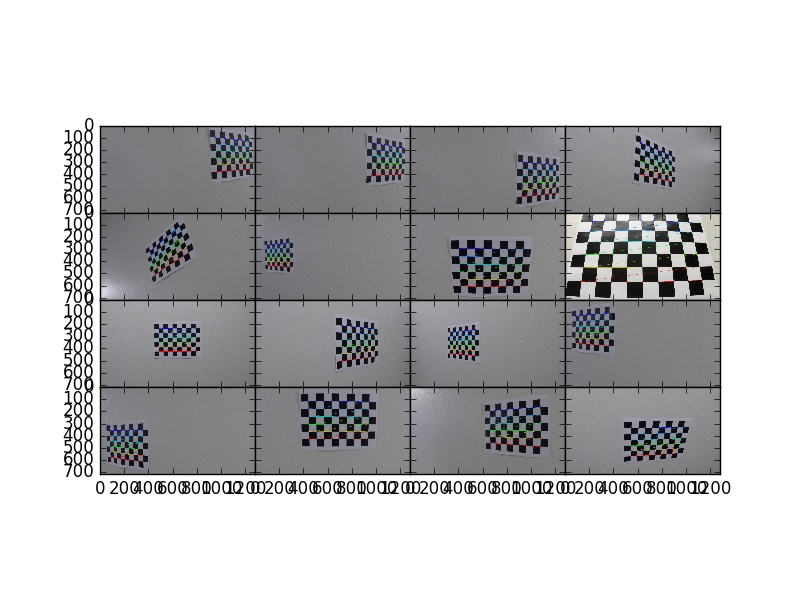
\includegraphics[width=.9\linewidth]{output_images/annotated_calibration_images.jpg}

\begin{verbatim}
def visualize(filename, a):
    fig, axes = plt.subplots(2,3,figsize=(24,12),subplot_kw={'xticks':[],'yticks':[]})
    fig.subplots_adjust(hspace=0.03, wspace=0.05)
    for p in zip(sum(axes.tolist(),[]), a):
	p[0].imshow(p[1],cmap='gray')
    plt.tight_layout()
    fig.savefig(filename)
    plt.close()
\end{verbatim}

\begin{verbatim}
visualize("output_images/test_images.jpg",
	  (mpimg.imread(f) for f in cycle(glob.glob("test_images/test*.jpg"))))
\end{verbatim}

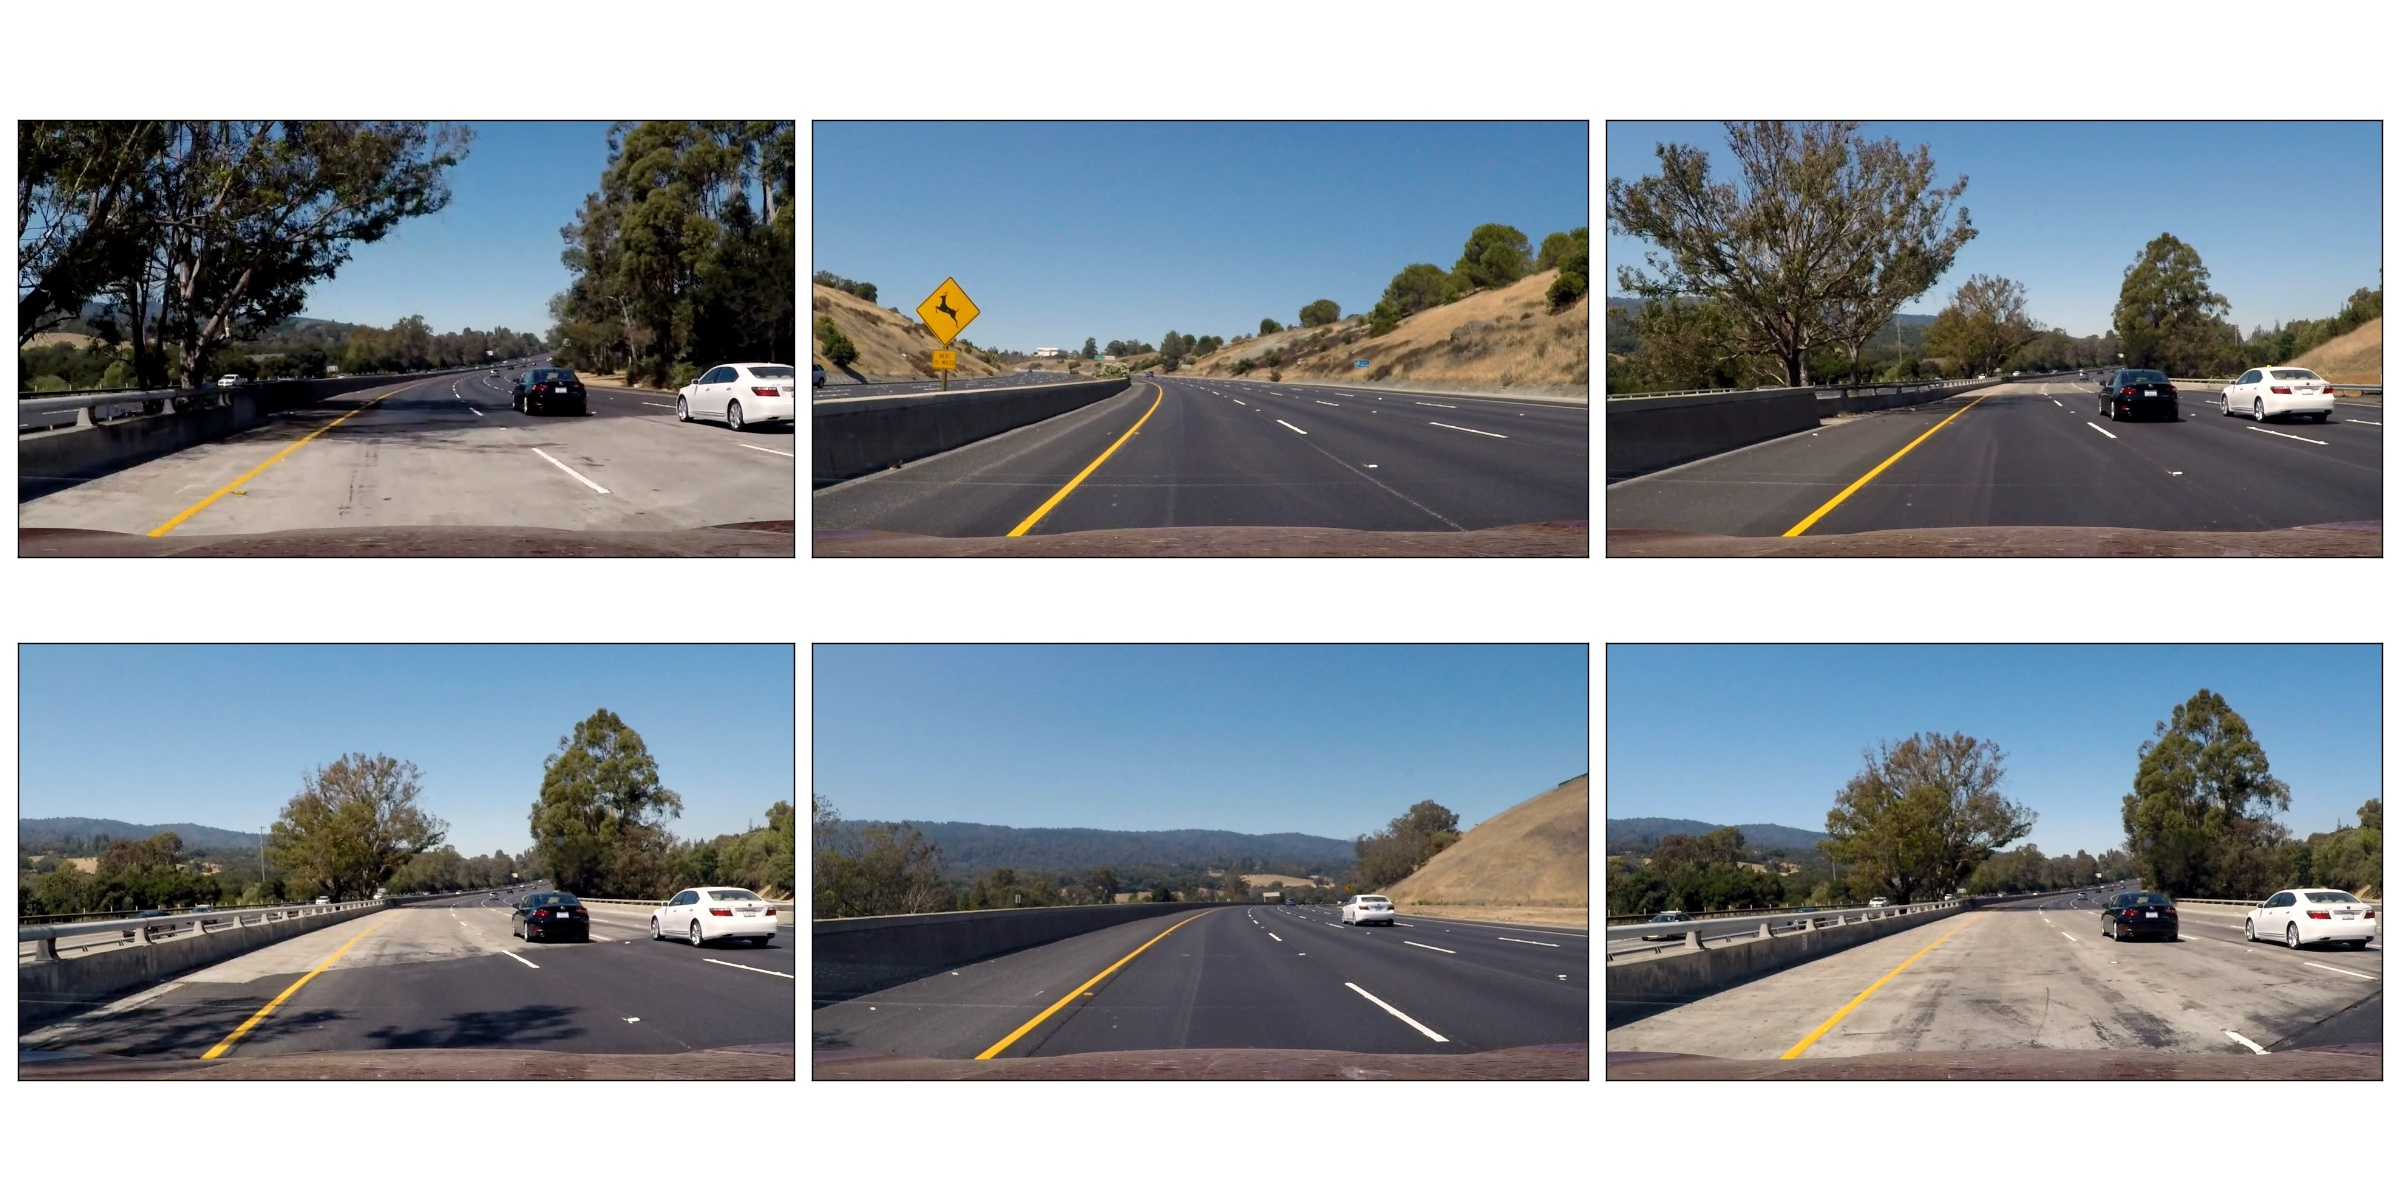
\includegraphics[width=.9\linewidth]{output_images/test_images.jpg}

\begin{verbatim}
visualize("output_images/undistorted_test_images.jpg",
	  (undistort(mpimg.imread(f)) for f in cycle(glob.glob("test_images/test*.jpg"))))
\end{verbatim}

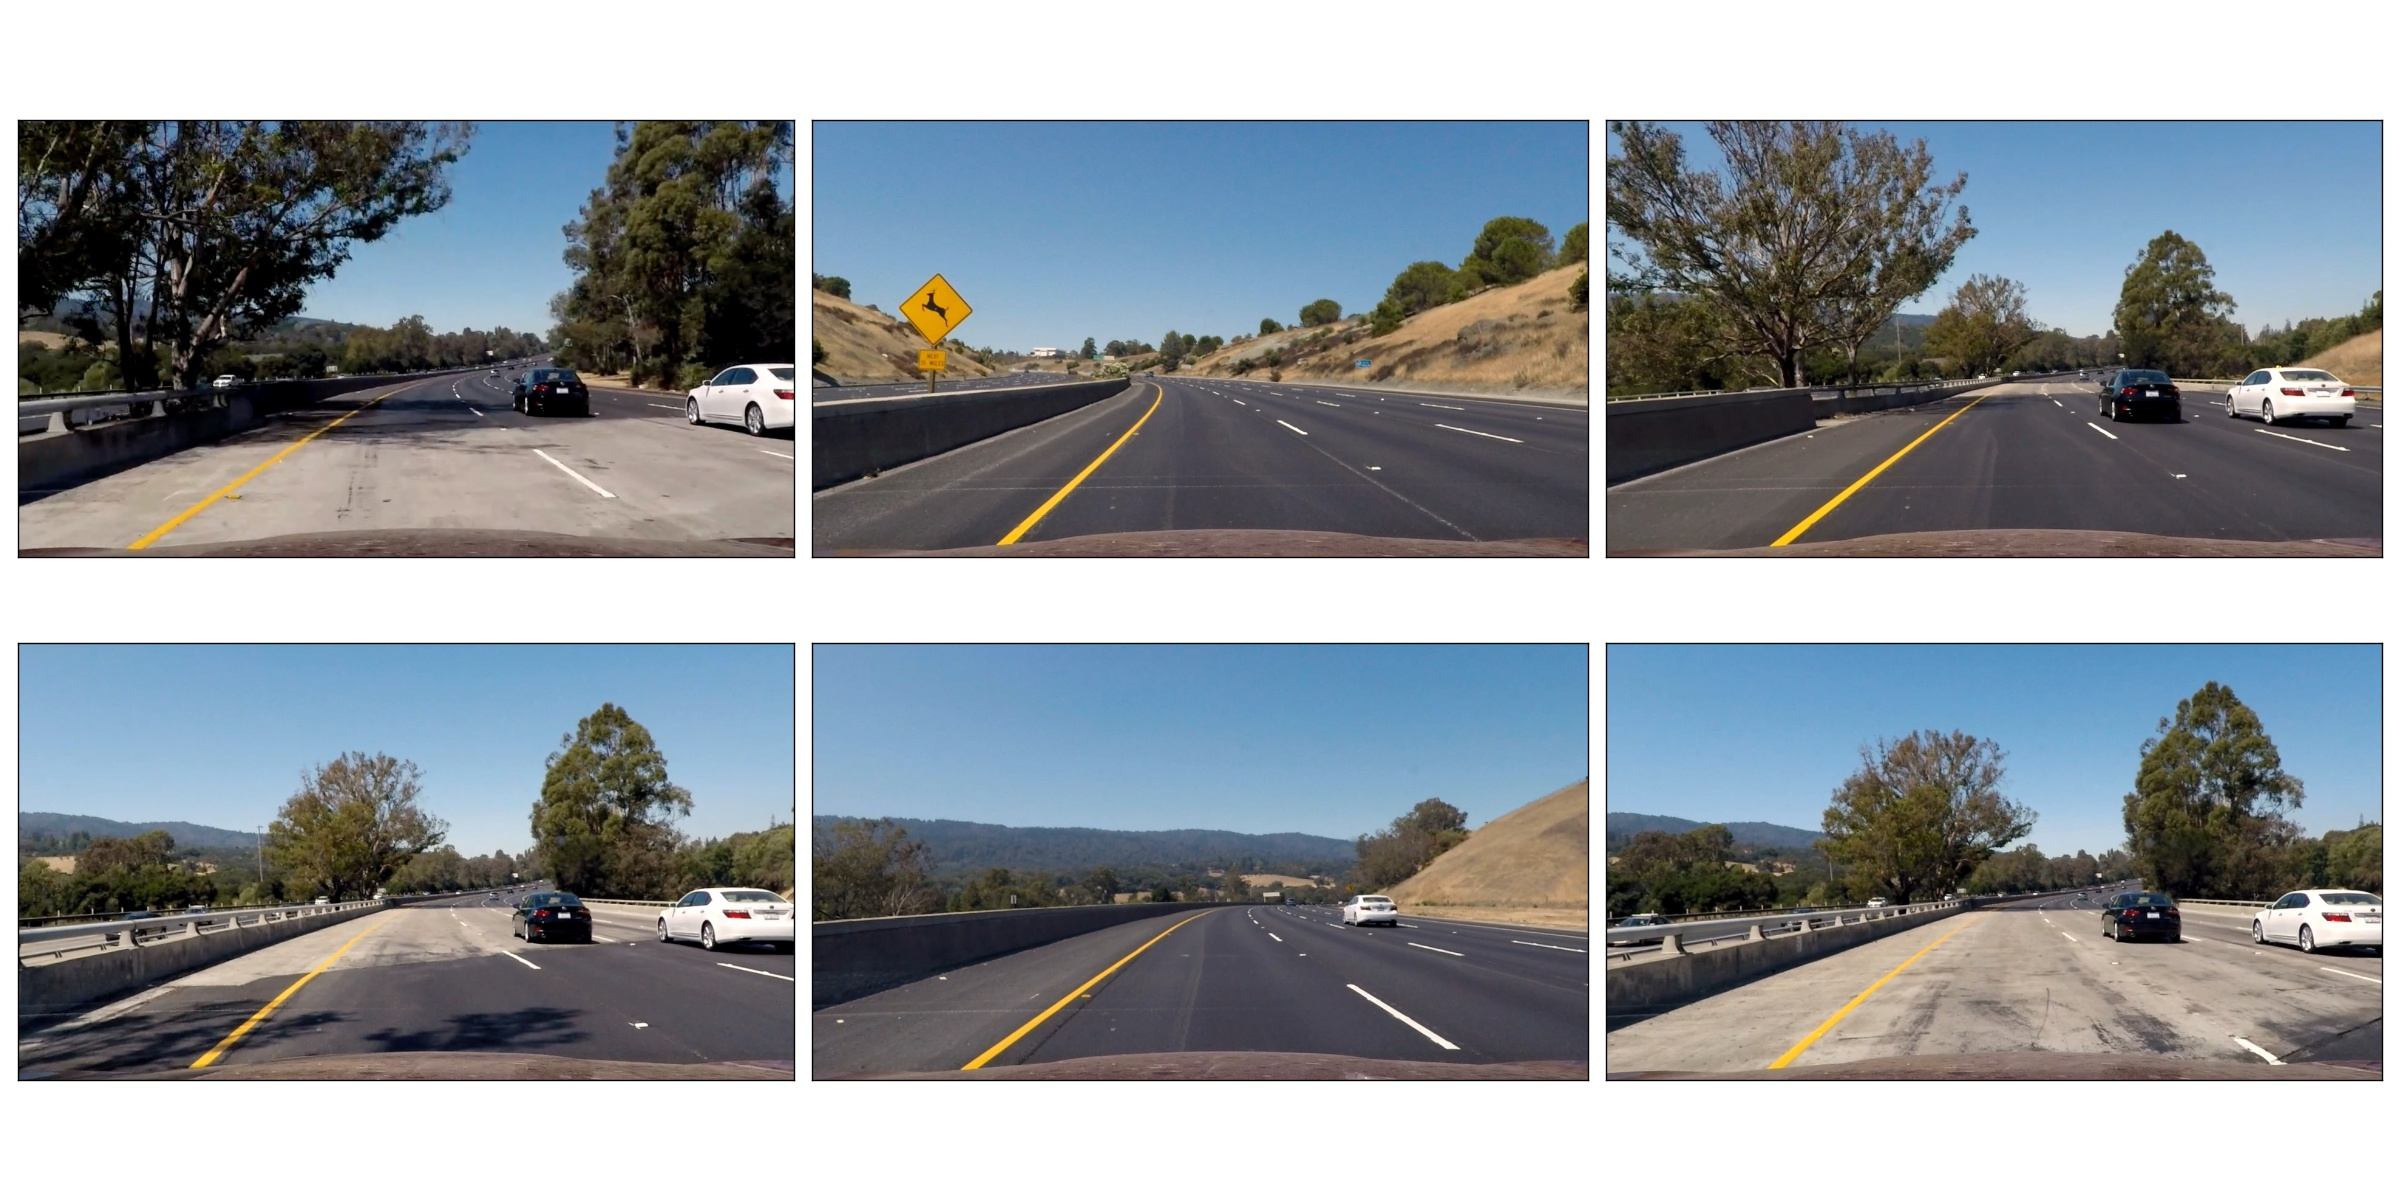
\includegraphics[width=.9\linewidth]{output_images/undistorted_test_images.jpg}

\subsubsection*{Perspective Measurement}
\label{sec-2-2-3}

\begin{verbatim}
def measure_warp(img):
    top = 0
    bottom = img.shape[0]
    def handler(e):
	if len(src)<4:
	    plt.axhline(int(e.ydata), linewidth=2, color='r')
	    plt.axvline(int(e.xdata), linewidth=2, color='r')
	    src.append((int(e.xdata),int(e.ydata)))
	if len(src)==4:
	    dst.extend([(300,bottom),(300,top),(980,top),(980,bottom)])
    was_interactive = matplotlib.is_interactive()
    if not matplotlib.is_interactive():
	plt.ion()
    fig = plt.figure()
    plt.imshow(img)
    global src
    global dst
    src = []
    dst = []
    cid1 = fig.canvas.mpl_connect('button_press_event', handler)
    cid2 = fig.canvas.mpl_connect('close_event', lambda e: e.canvas.stop_event_loop())
    fig.canvas.start_event_loop(timeout=-1)
    M = cv2.getPerspectiveTransform(np.asfarray(src, np.float32), np.asfarray(dst, np.float32))
    Minv = cv2.getPerspectiveTransform(np.asfarray(dst, np.float32), np.asfarray(src, np.float32))
    matplotlib.interactive(was_interactive)
    return M, Minv
\end{verbatim}

\begin{verbatim}
def get_warpers(corrected_image):
    M, Minv = measure_warp(corrected_image)
    return lambda x: cv2.warpPerspective(x, M, x.shape[:2][::-1], flags=cv2.INTER_LINEAR), lambda x: cv2.warpPerspective(x, Minv, x.shape[:2][::-1], flags=cv2.INTER_LINEAR), M, Minv
\end{verbatim}

\begin{verbatim}
warp,unwarp,M,Minv = get_warpers(undistort(mpimg.imread("test_images/straight_lines2.jpg")))
\end{verbatim}

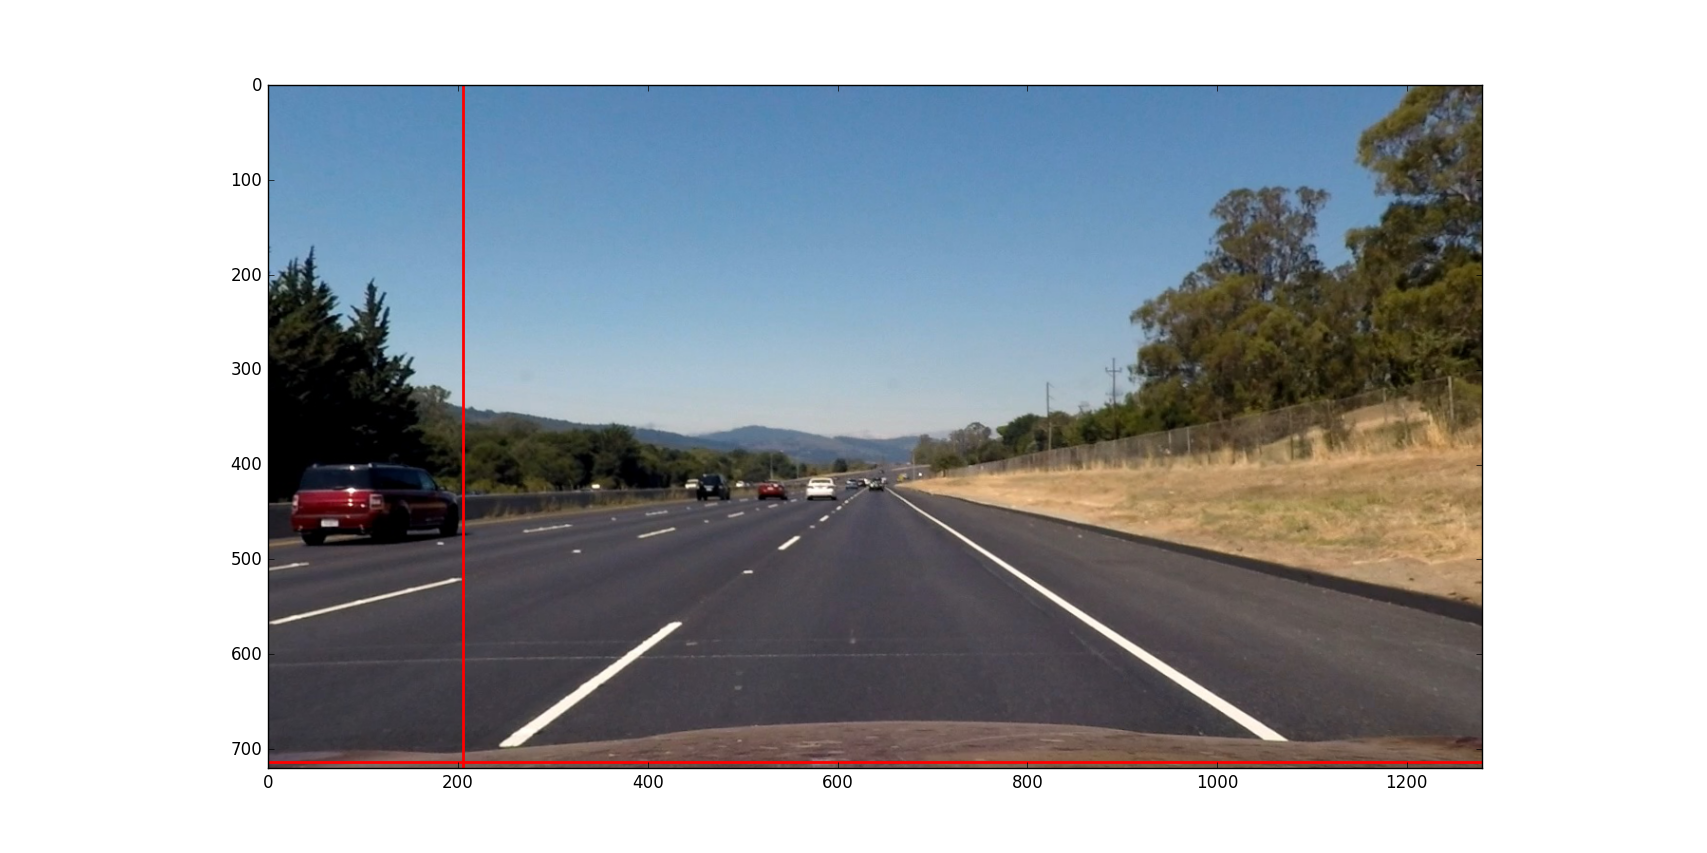
\includegraphics[width=.9\linewidth]{output_images/figure_3-1.png}

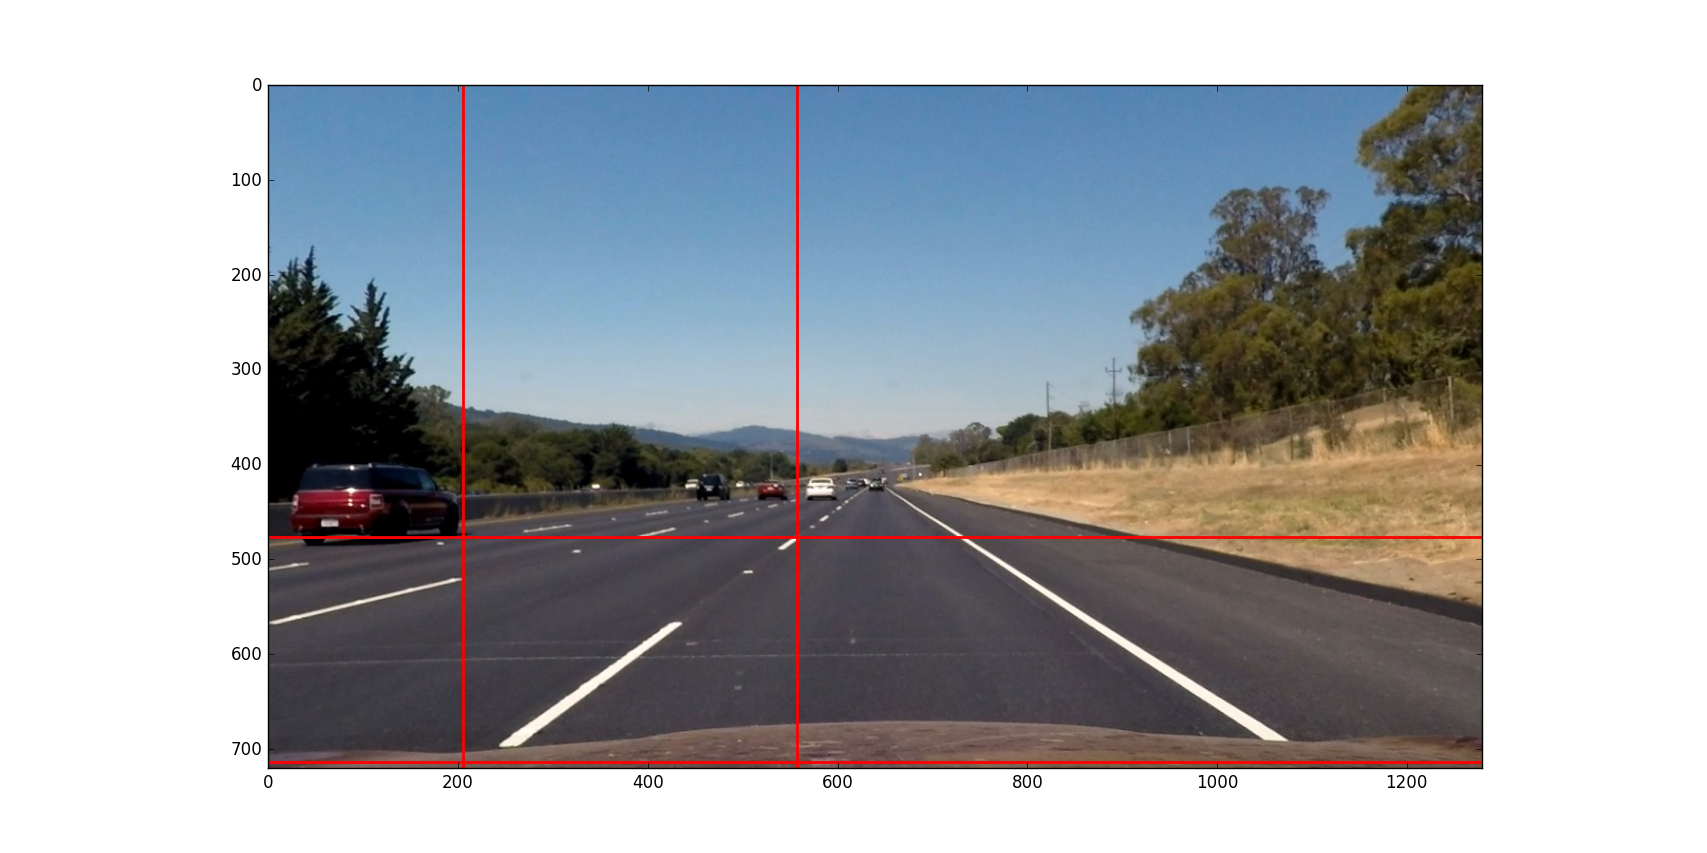
\includegraphics[width=.9\linewidth]{output_images/figure_3-2.png}

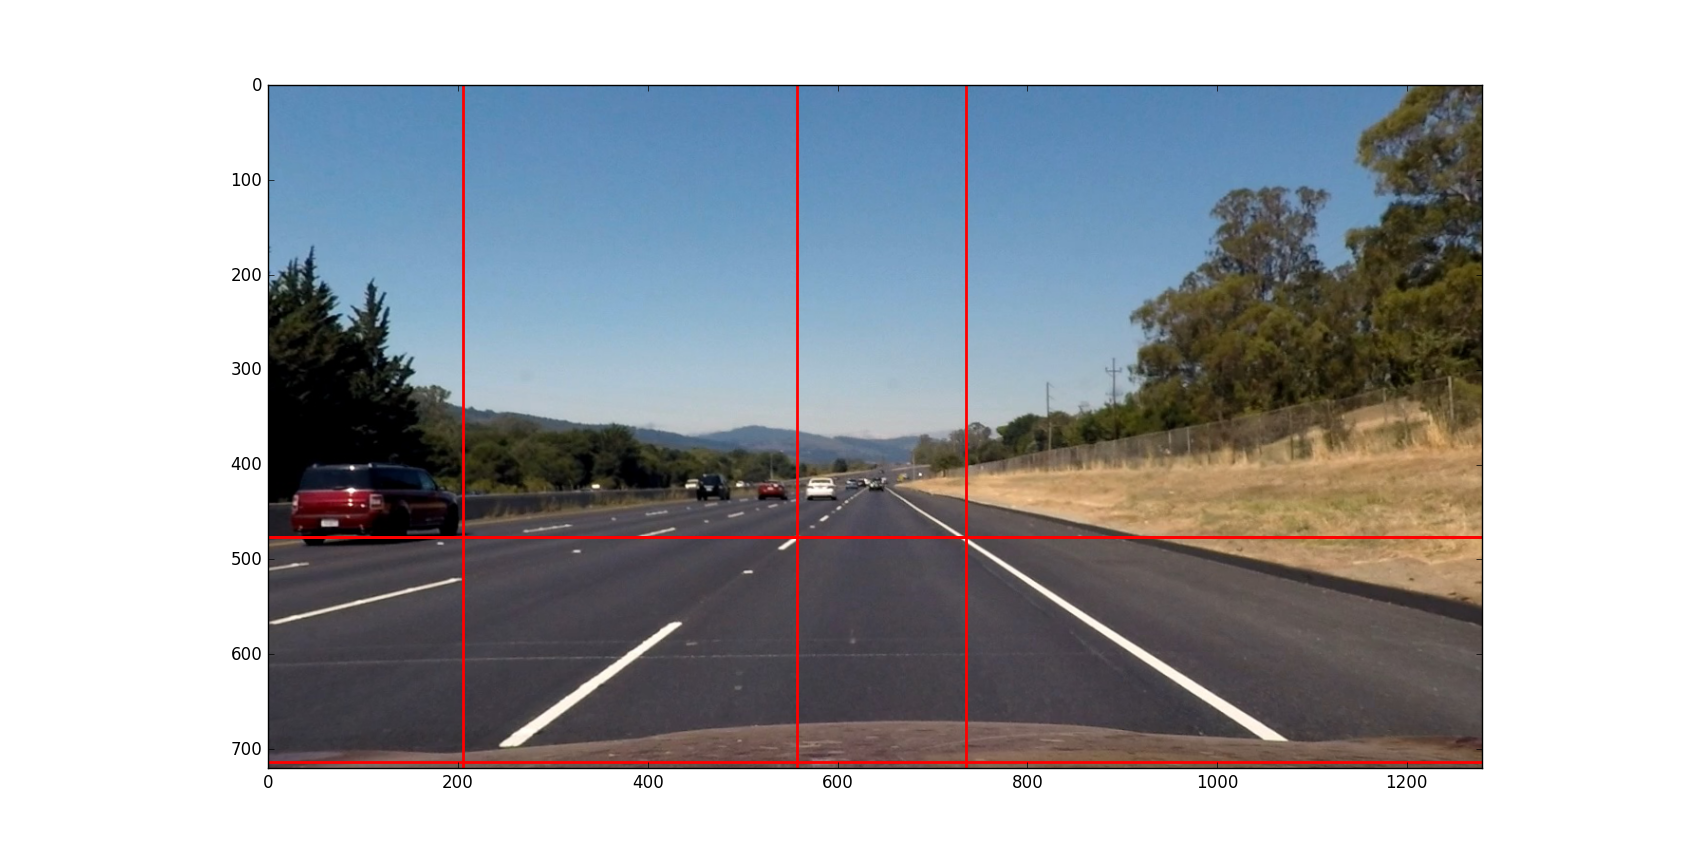
\includegraphics[width=.9\linewidth]{output_images/figure_3-3.png}

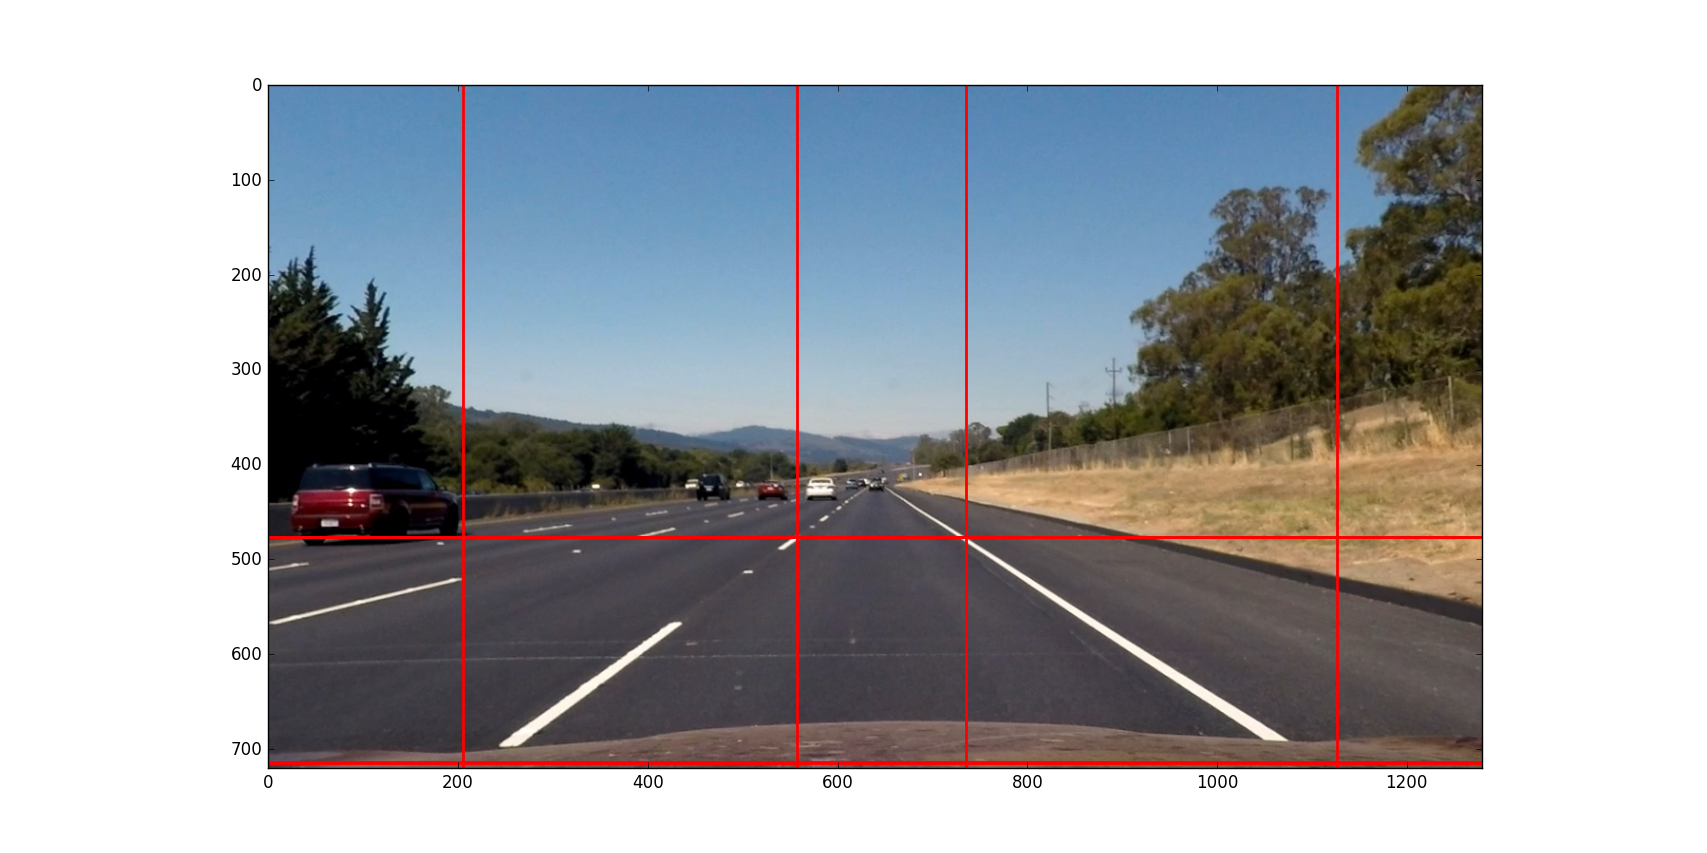
\includegraphics[width=.9\linewidth]{output_images/figure_3-4.png}

\begin{verbatim}
visualize("output_images/warped_undistorted_test_images.jpg",
	  (warp(undistort(mpimg.imread(f))) for f in cycle(glob.glob("test_images/test*.jpg"))))
\end{verbatim}

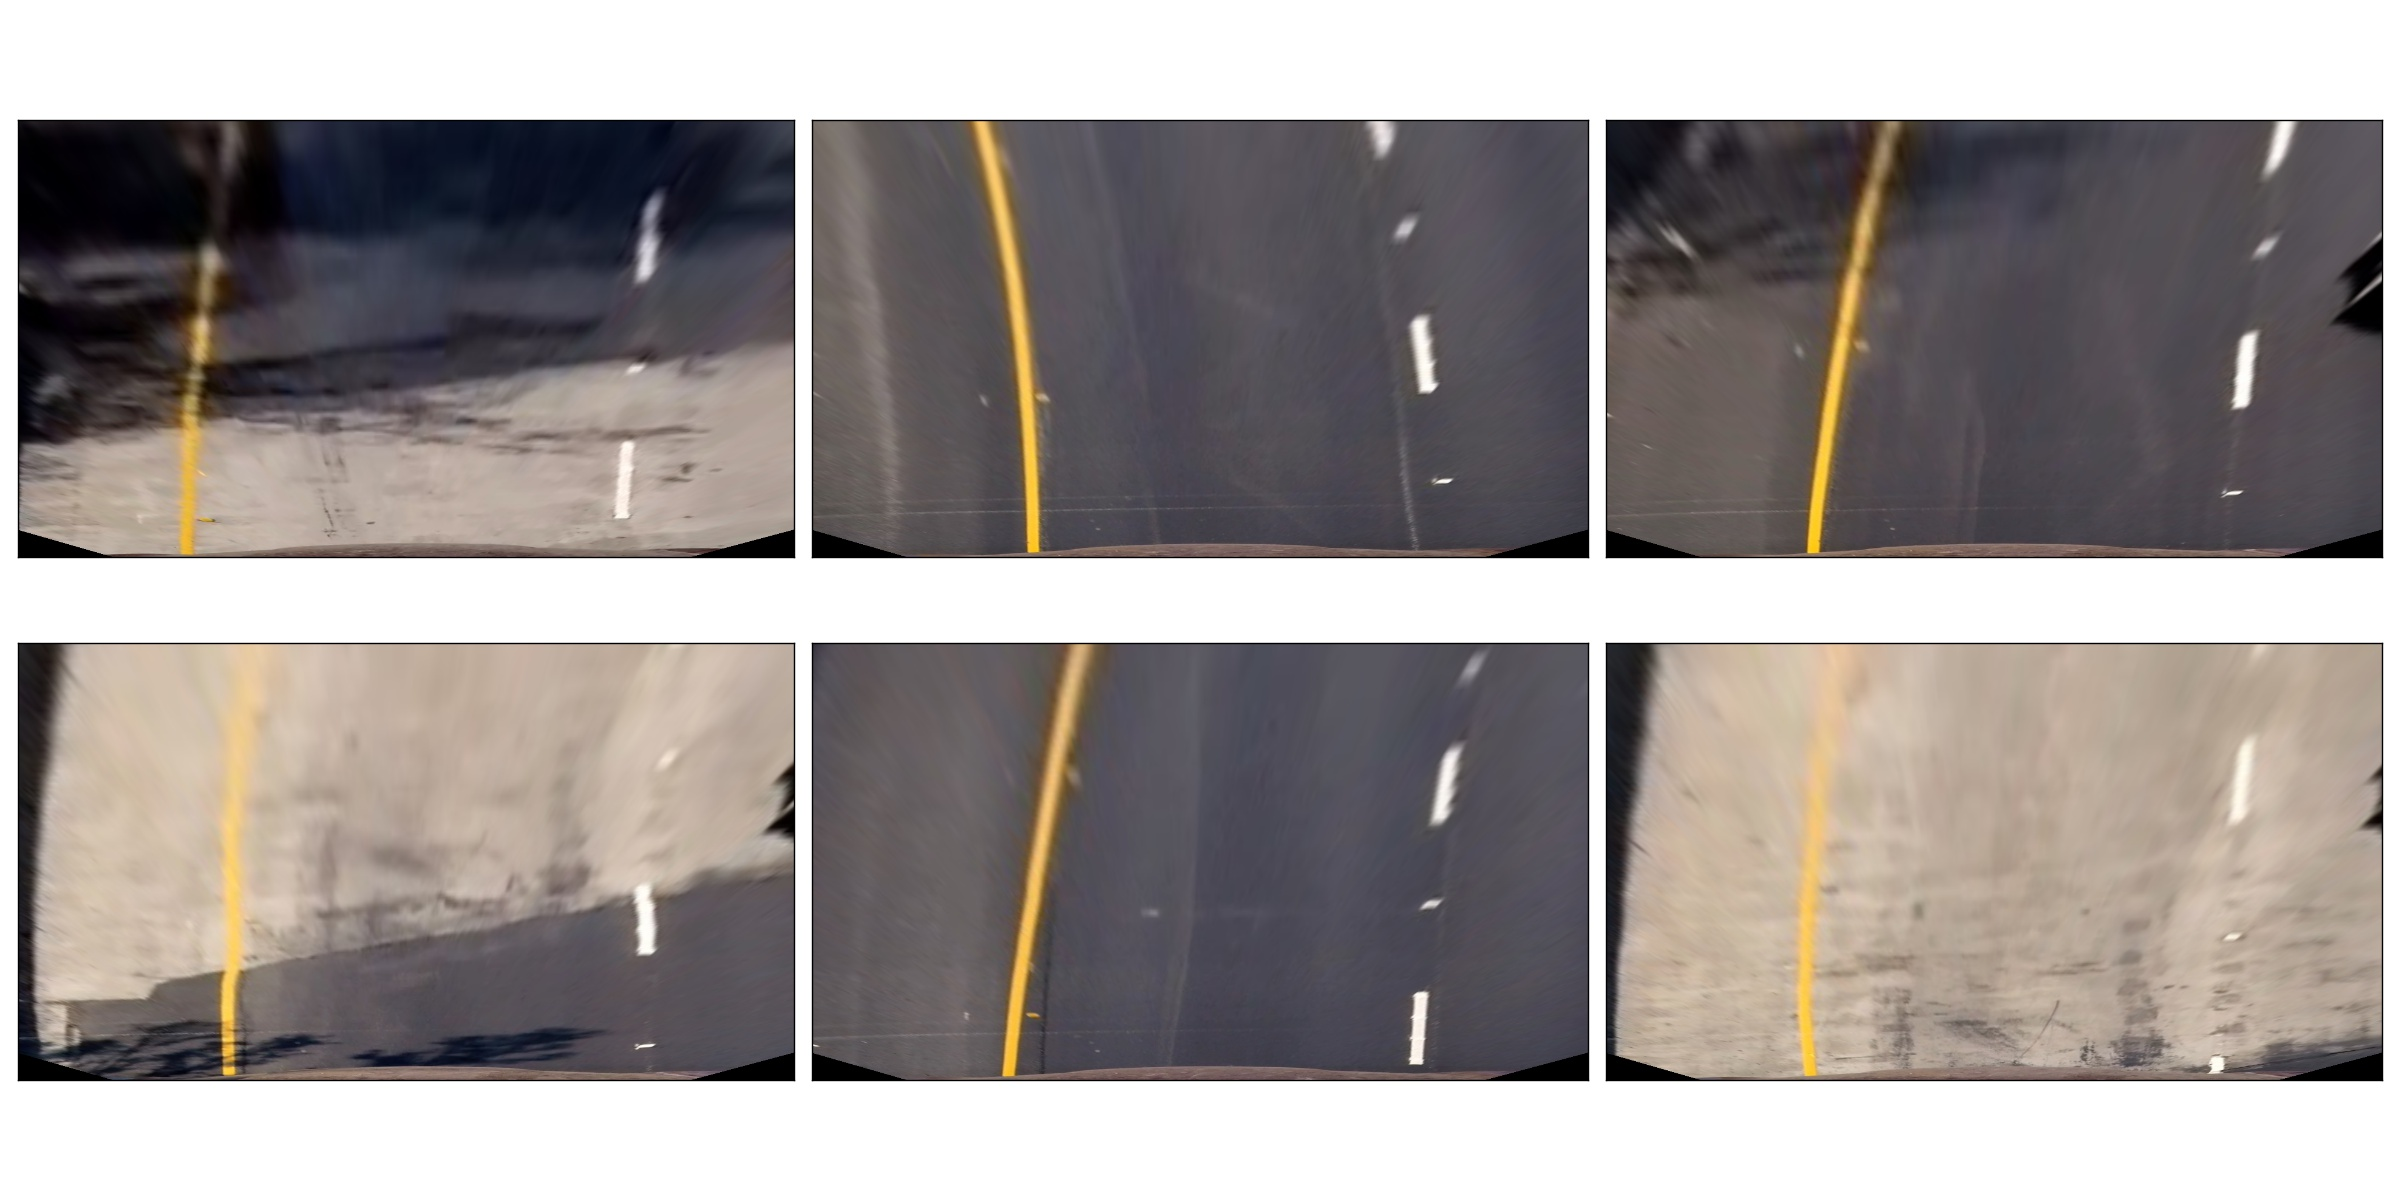
\includegraphics[width=.9\linewidth]{output_images/warped_undistorted_test_images.jpg}


\subsection*{Pipeline}
\label{sec-2-3}

\subsubsection*{Gradient and Color Thresholds}
\label{sec-2-3-1}

\begin{verbatim}
def scale(img, factor=255.0):
    scale_factor = np.max(img)/factor
    return (img/scale_factor).astype(np.uint8)
\end{verbatim}

\begin{verbatim}
def derivative(img, sobel_kernel=3):
    derivx = np.absolute(cv2.Sobel(img, cv2.CV_64F, 1, 0, ksize=sobel_kernel))
    derivy = np.absolute(cv2.Sobel(img, cv2.CV_64F, 0, 1, ksize=sobel_kernel))
    gradmag = np.sqrt(derivx**2 + derivy**2)
    absgraddir = np.arctan2(derivy, derivx)
    return scale(derivx), scale(derivy), scale(gradmag), absgraddir
\end{verbatim}

\begin{verbatim}
def grad(img, k1=3, k2=15):
    _,_,g,_ = derivative(img, sobel_kernel=k1)
    _,_,_,p = derivative(img, sobel_kernel=k2)
    return g,p
\end{verbatim}

\begin{verbatim}
def hls_select(img):
    hsv = cv2.cvtColor(img, cv2.COLOR_RGB2HLS).astype(np.float)
    h = hsv[:,:,0]
    l = hsv[:,:,1]
    s = hsv[:,:,2]
    return h,l,s
\end{verbatim}

\begin{verbatim}
def rgb_select(img):
    rgb = img
    r = rgb[:,:,0]
    g = rgb[:,:,1]
    b = rgb[:,:,2]
    return r,g,b
\end{verbatim}

\begin{verbatim}
def threshold(img, thresh_min=0, thresh_max=255):
    binary_output = np.zeros_like(img)
    binary_output[(img >= thresh_min) & (img <= thresh_max)] = 1
    return binary_output
\end{verbatim}

\begin{verbatim}
land = lambda *x: np.logical_and.reduce(x)
lor = lambda *x: np.logical_or.reduce(x)
\end{verbatim}

\begin{verbatim}
def highlight(img):
    r,g,b = rgb_select(img)
    h,l,s = hls_select(img)
    o01 = threshold(r, 200, 255)
    o02 = threshold(g, 200, 255)
    o03 = threshold(s, 200, 255)
    return scale(lor(land(o01,o02),o03))
\end{verbatim}

\begin{verbatim}
visualize("output_images/binary_undistorted_test_images.jpg",
	  (highlight(undistort(mpimg.imread(f))) for f in cycle(glob.glob("test_images/test*.jpg"))))
\end{verbatim}

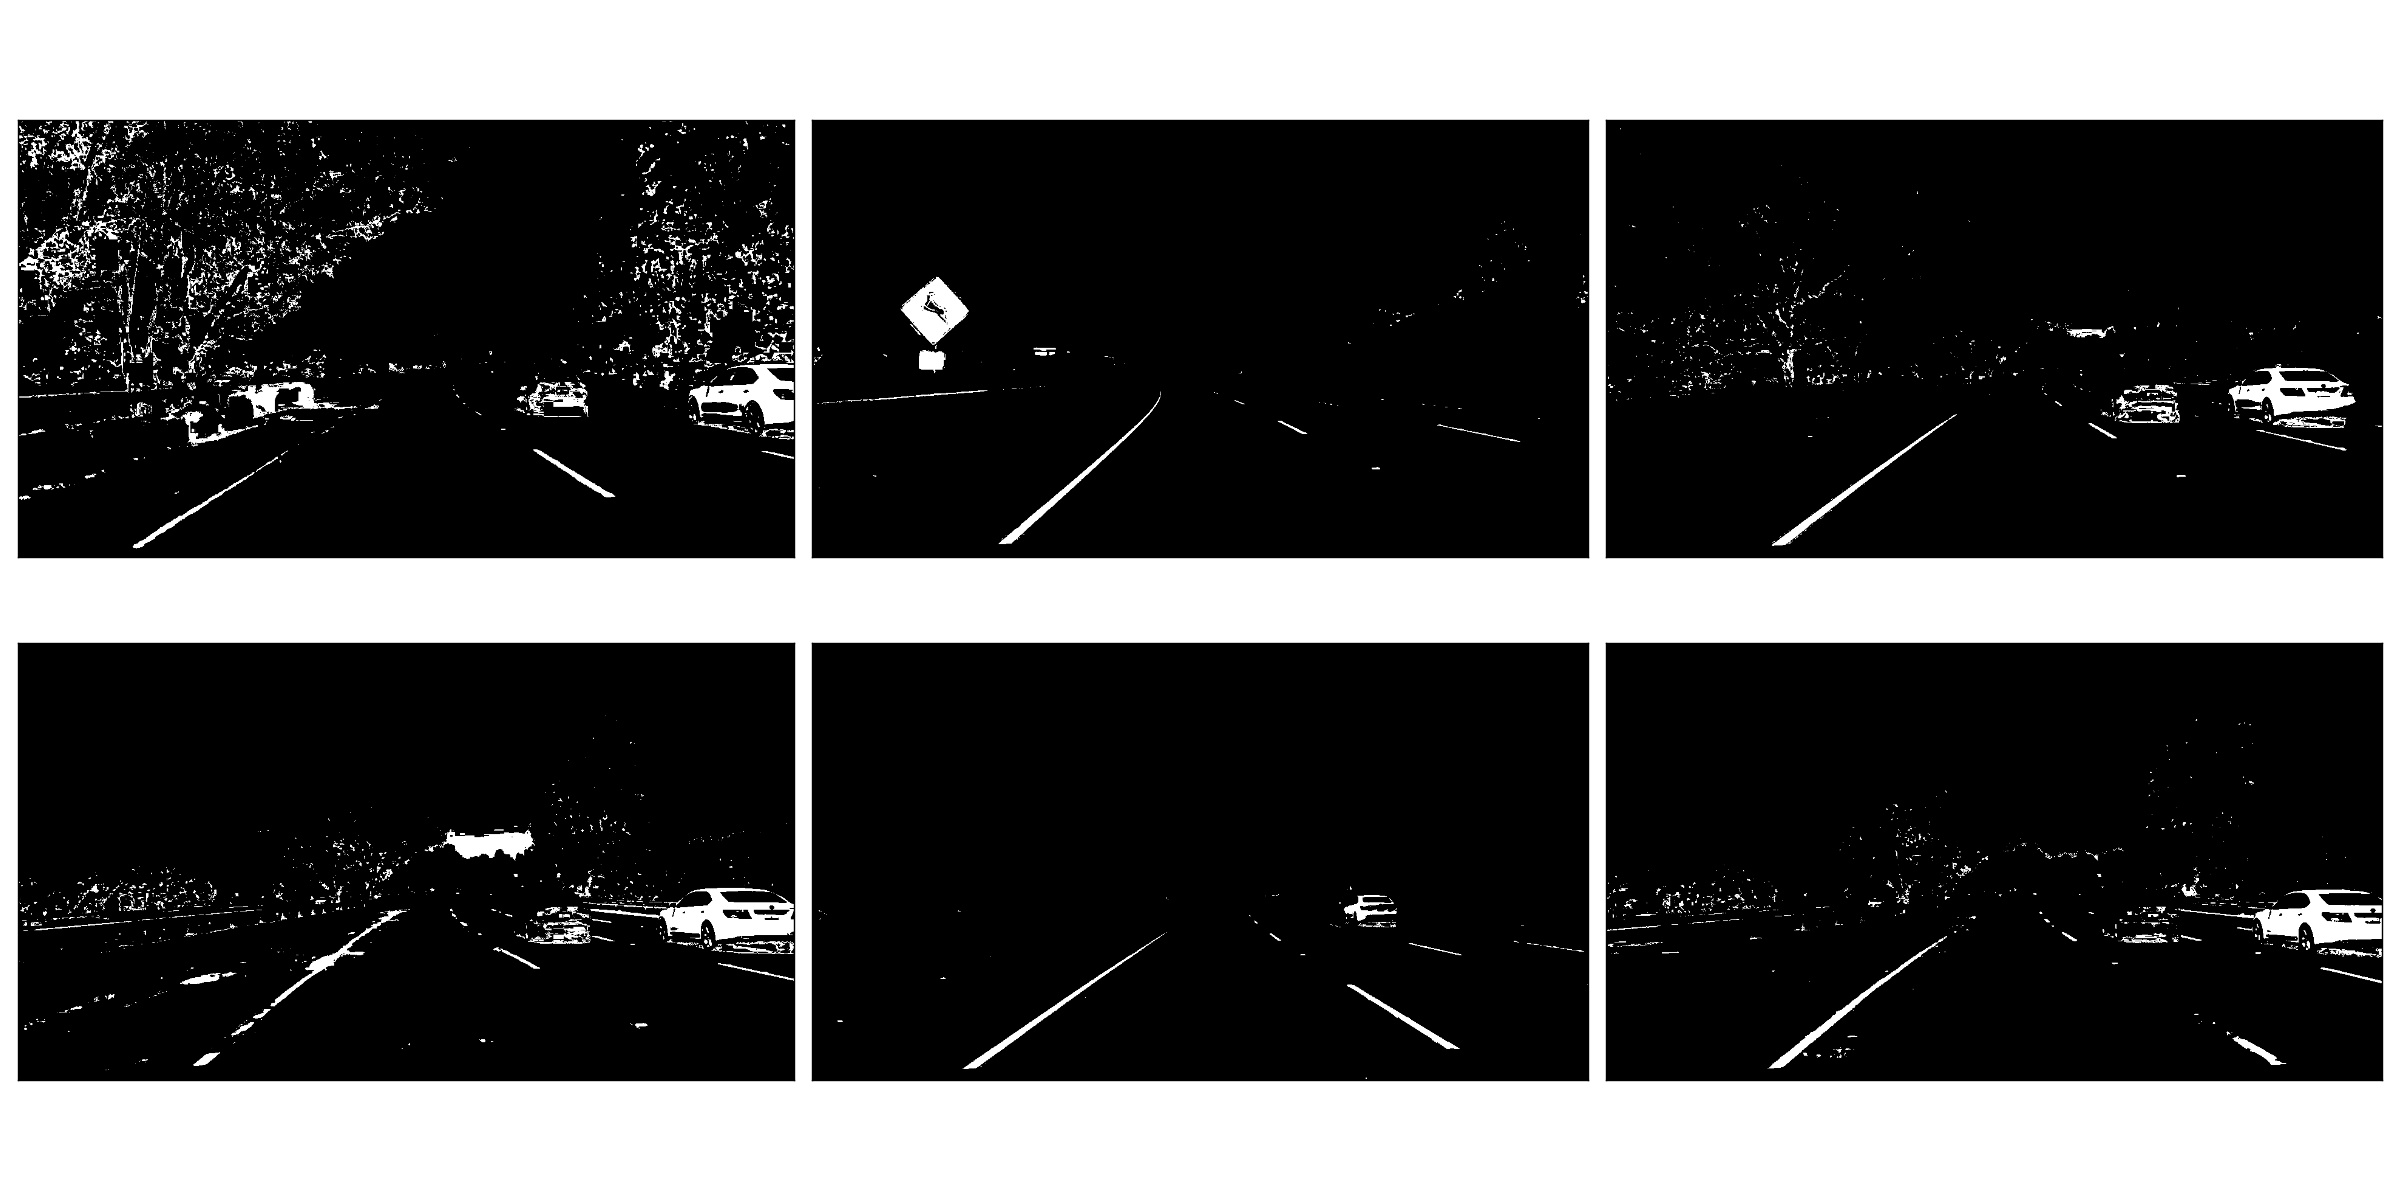
\includegraphics[width=.9\linewidth]{output_images/binary_undistorted_test_images.jpg}

\subsubsection*{Perspective Transform}
\label{sec-2-3-2}

\begin{verbatim}
visualize("output_images/warped_binary_undistorted_images.jpg",
	  (warp(highlight(undistort(mpimg.imread(f)))) for f in cycle(glob.glob("test_images/test*.jpg"))))
\end{verbatim}

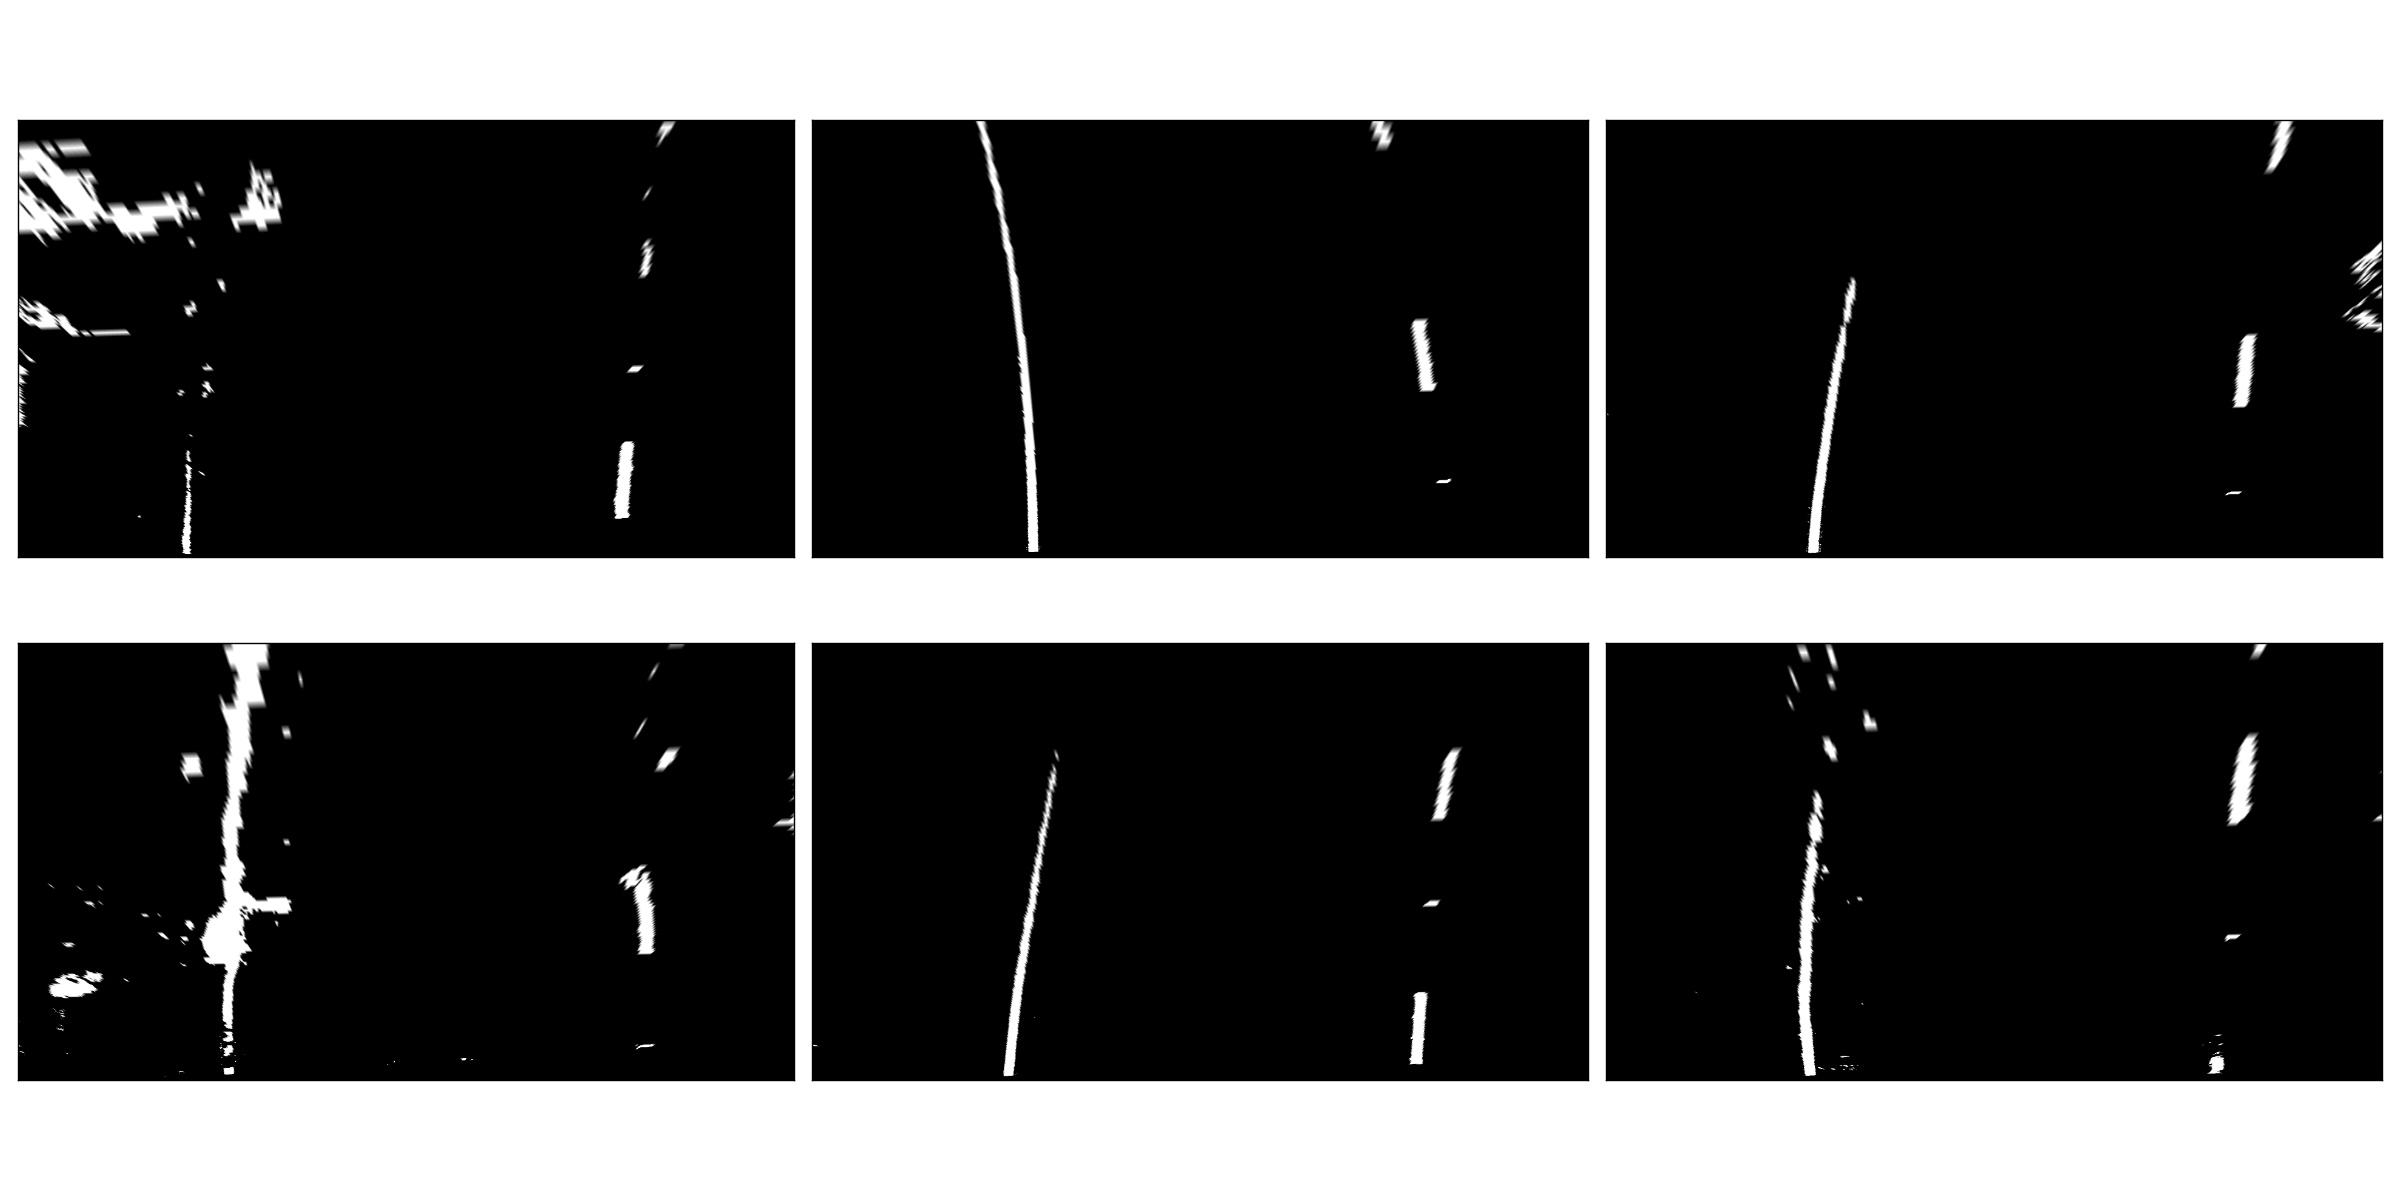
\includegraphics[width=.9\linewidth]{output_images/warped_binary_undistorted_images.jpg}

\subsubsection*{Lane-Finding}
\label{sec-2-3-3}

\begin{verbatim}
def detect_lines_sliding_window(warped_binary):
    # Assuming you have created a warped binary image called "warped_binary"
    # Take a histogram of the bottom half of the image
    histogram = np.sum(warped_binary[warped_binary.shape[0]/2:,:], axis=0)
    # Create an output image to draw on and  visualize the result
    out_img = np.dstack((warped_binary, warped_binary, warped_binary))*255
    # Find the peak of the left and right halves of the histogram
    # These will be the starting point for the left and right lines
    midpoint = np.int(histogram.shape[0]/2)
    leftx_base = np.argmax(histogram[:midpoint])
    rightx_base = np.argmax(histogram[midpoint:]) + midpoint
    # Choose the number of sliding windows
    nwindows = 9
    # Set height of windows
    window_height = np.int(warped_binary.shape[0]/nwindows)
    # Identify the x and y positions of all nonzero pixels in the image
    nonzero = warped_binary.nonzero()
    nonzeroy = np.array(nonzero[0])
    nonzerox = np.array(nonzero[1])
    # Current positions to be updated for each window
    leftx_current = leftx_base
    rightx_current = rightx_base
    # Set the width of the windows +/- margin
    margin = 100
    # Set minimum number of pixels found to recenter window
    minpix = 50
    # Create empty lists to receive left and right lane pixel indices
    left_lane_inds = []
    right_lane_inds = []
    # Step through the windows one by one
    for window in range(nwindows):
	# Identify window boundaries in x and y (and right and left)
	win_y_low = warped_binary.shape[0] - (window+1)*window_height
	win_y_high = warped_binary.shape[0] - window*window_height
	win_xleft_low = leftx_current - margin
	win_xleft_high = leftx_current + margin
	win_xright_low = rightx_current - margin
	win_xright_high = rightx_current + margin
	# Draw the windows on the visualization image
	cv2.rectangle(out_img,(win_xleft_low,win_y_low),(win_xleft_high,win_y_high),(0,255,0), 2) 
	cv2.rectangle(out_img,(win_xright_low,win_y_low),(win_xright_high,win_y_high),(0,255,0), 2) 
	# Identify the nonzero pixels in x and y within the window
	good_left_inds = ((nonzeroy >= win_y_low) & (nonzeroy < win_y_high) & (nonzerox >= win_xleft_low) & (nonzerox < win_xleft_high)).nonzero()[0]
	good_right_inds = ((nonzeroy >= win_y_low) & (nonzeroy < win_y_high) & (nonzerox >= win_xright_low) & (nonzerox < win_xright_high)).nonzero()[0]
	# Append these indices to the lists
	left_lane_inds.append(good_left_inds)
	right_lane_inds.append(good_right_inds)
	# If you found > minpix pixels, recenter next window on their mean position
	if len(good_left_inds) > minpix:
	    leftx_current = np.int(np.mean(nonzerox[good_left_inds]))
	if len(good_right_inds) > minpix:        
	    rightx_current = np.int(np.mean(nonzerox[good_right_inds]))
    # Concatenate the arrays of indices
    left_lane_inds = np.concatenate(left_lane_inds)
    right_lane_inds = np.concatenate(right_lane_inds)
    # Extract left and right line pixel positions
    leftx = nonzerox[left_lane_inds]
    lefty = nonzeroy[left_lane_inds] 
    rightx = nonzerox[right_lane_inds]
    righty = nonzeroy[right_lane_inds] 
    # Fit a second order polynomial to each
    left_fit,left_res,_,_,_ = np.polyfit(lefty, leftx, 2, full=True)
    right_fit,right_res,_,_,_ = np.polyfit(righty, rightx, 2, full=True)
    # Generate x and y values for plotting
    ploty = np.linspace(0, warped_binary.shape[0]-1, warped_binary.shape[0] )
    left_fitx = left_fit[0]*ploty**2 + left_fit[1]*ploty + left_fit[2]
    right_fitx = right_fit[0]*ploty**2 + right_fit[1]*ploty + right_fit[2]
    out_img[nonzeroy[left_lane_inds], nonzerox[left_lane_inds]] = [255, 0, 0]
    out_img[nonzeroy[right_lane_inds], nonzerox[right_lane_inds]] = [0, 0, 255]
    out_img[ploty.astype('int'),left_fitx.astype('int')] = [0, 255, 255]
    out_img[ploty.astype('int'),right_fitx.astype('int')] = [0, 255, 255]
    y_eval = warped_binary.shape[0]
    # Define conversions in x and y from pixels space to meters
    ym_per_pix = 30/720 # meters per pixel in y dimension
    xm_per_pix = 3.7/700 # meters per pixel in x dimension
    # Fit new polynomials to x,y in world space
    left_fit_cr = np.polyfit(lefty*ym_per_pix, leftx*xm_per_pix, 2)
    right_fit_cr = np.polyfit(righty*ym_per_pix, rightx*xm_per_pix, 2)
    # Calculate the new radii of curvature
    left_curverad = ((1 + (2*left_fit_cr[0]*y_eval*ym_per_pix + left_fit_cr[1])**2)**1.5) / np.absolute(2*left_fit_cr[0])
    right_curverad = ((1 + (2*right_fit_cr[0]*y_eval*ym_per_pix + right_fit_cr[1])**2)**1.5) / np.absolute(2*right_fit_cr[0])
    return left_fit, right_fit, np.sqrt(left_fit[1]/len(leftx)), np.sqrt(right_fit[1]/len(rightx)), left_curverad, right_curverad, out_img
\end{verbatim}

\begin{verbatim}
visualize("output_images/detected_lines_test_images.jpg",
	  (detect_lines_sliding_window(warp(highlight(undistort(mpimg.imread(f)))))[6] for f in cycle(glob.glob("test_images/test*.jpg"))))
\end{verbatim}

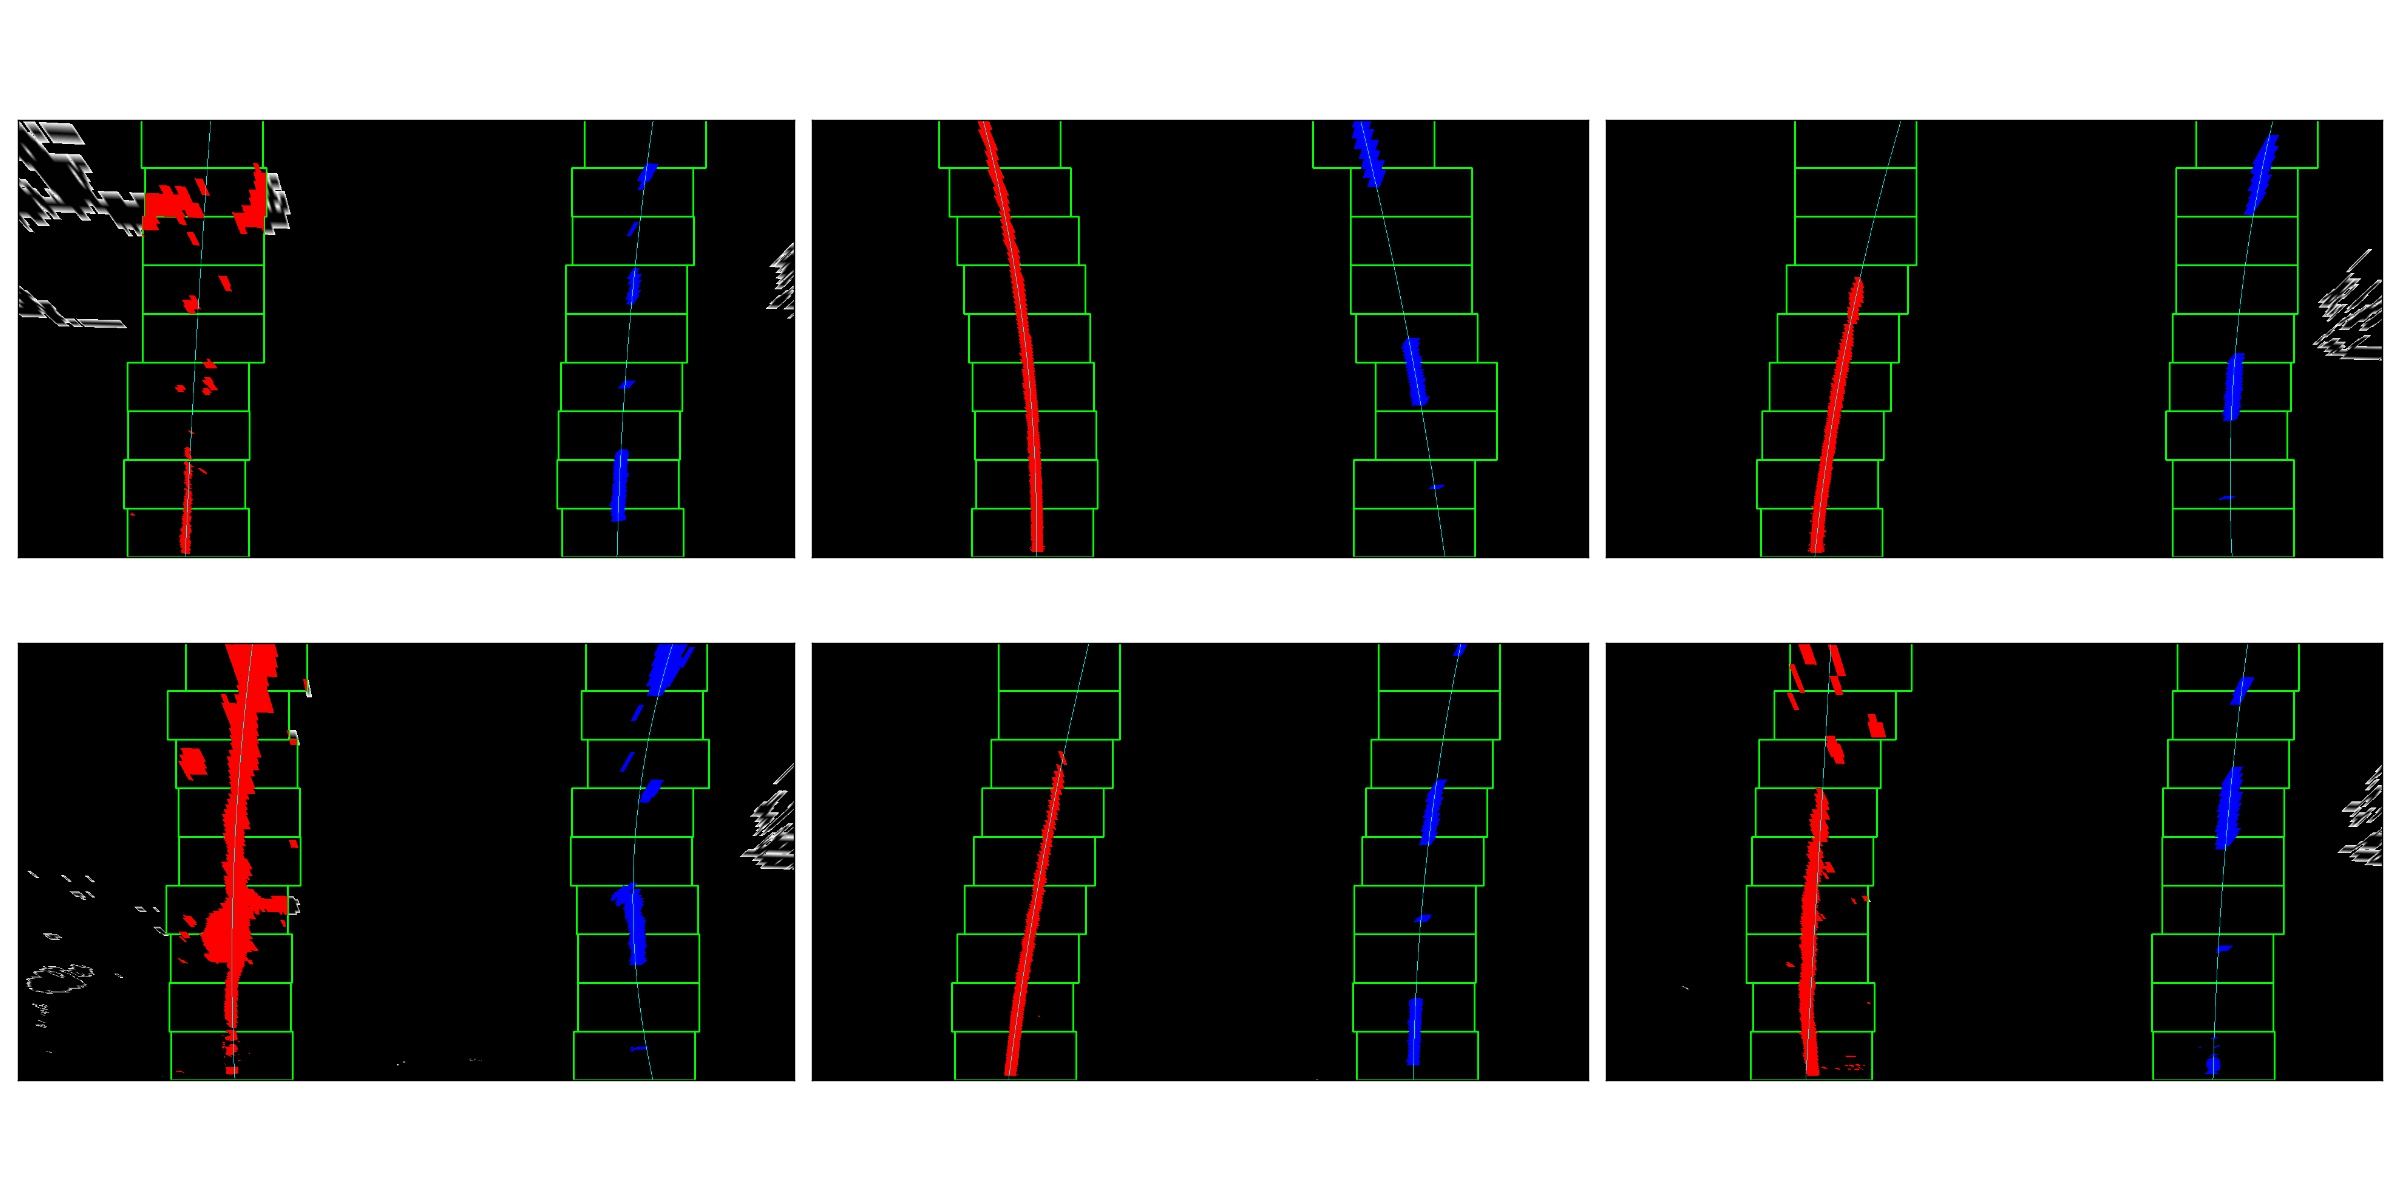
\includegraphics[width=.9\linewidth]{output_images/detected_lines_test_images.jpg}

\begin{verbatim}
def detect_lines(warped_binary, left_fit, right_fit):
    # from the next frame of video (also called "binary_warped")
    # It's now much easier to find line pixels!
    nonzero = warped_binary.nonzero()
    nonzeroy = np.array(nonzero[0])
    nonzerox = np.array(nonzero[1])
    margin = 100
    left_lane_inds = ((nonzerox > (left_fit[0]*(nonzeroy**2) + left_fit[1]*nonzeroy + left_fit[2] - margin)) & (nonzerox < (left_fit[0]*(nonzeroy**2) + left_fit[1]*nonzeroy + left_fit[2] + margin))) 
    right_lane_inds = ((nonzerox > (right_fit[0]*(nonzeroy**2) + right_fit[1]*nonzeroy + right_fit[2] - margin)) & (nonzerox < (right_fit[0]*(nonzeroy**2) + right_fit[1]*nonzeroy + right_fit[2] + margin)))  
    # Again, extract left and right line pixel positions
    leftx = nonzerox[left_lane_inds]
    lefty = nonzeroy[left_lane_inds] 
    rightx = nonzerox[right_lane_inds]
    righty = nonzeroy[right_lane_inds]
    # Fit a second order polynomial to each
    left_fit,left_res,_,_,_ = np.polyfit(lefty, leftx, 2, full=True)
    right_fit,right_res,_,_,_ = np.polyfit(righty, rightx, 2, full=True)
    # Generate x and y values for plotting
    ploty = np.linspace(0, warped_binary.shape[0]-1, warped_binary.shape[0] )
    left_fitx = left_fit[0]*ploty**2 + left_fit[1]*ploty + left_fit[2]
    right_fitx = right_fit[0]*ploty**2 + right_fit[1]*ploty + right_fit[2]
    y_eval = warped_binary.shape[0]
    # Define conversions in x and y from pixels space to meters
    ym_per_pix = 30/720 # meters per pixel in y dimension
    xm_per_pix = 3.7/700 # meters per pixel in x dimension
    # Fit new polynomials to x,y in world space
    left_fit_cr = np.polyfit(lefty*ym_per_pix, leftx*xm_per_pix, 2)
    right_fit_cr = np.polyfit(righty*ym_per_pix, rightx*xm_per_pix, 2)
    # Calculate the new radii of curvature
    left_curverad = ((1 + (2*left_fit_cr[0]*y_eval*ym_per_pix + left_fit_cr[1])**2)**1.5) / np.absolute(2*left_fit_cr[0])
    right_curverad = ((1 + (2*right_fit_cr[0]*y_eval*ym_per_pix + right_fit_cr[1])**2)**1.5) / np.absolute(2*right_fit_cr[0])
    return left_fit, right_fit, np.sqrt(left_fit[1]/len(leftx)), np.sqrt(right_fit[1]/len(rightx)), left_curverad, right_curverad, None
\end{verbatim}

\begin{verbatim}
def draw_lane(undistorted, warped_binary, l_fit, r_fit, l_rad, r_rad, unwarp):
    # Create an image to draw the lines on
    warp_zero = np.zeros_like(warped_binary).astype(np.uint8)
    color_warp = np.dstack((warp_zero, warp_zero, warp_zero))
    # Generate x and y values for plotting
    ploty = np.linspace(0, warped_binary.shape[0]-1, warped_binary.shape[0])
    l_fitx = l_fit[0]*ploty**2 + l_fit[1]*ploty + l_fit[2]
    r_fitx = r_fit[0]*ploty**2 + r_fit[1]*ploty + r_fit[2]
    # Recast the x and y points into usable format for cv2.fillPoly()
    pts_left = np.array([np.transpose(np.vstack([l_fitx, ploty]))])
    pts_right = np.array([np.flipud(np.transpose(np.vstack([r_fitx, ploty])))])
    pts = np.hstack((pts_left, pts_right))
    # Draw the lane onto the warped_binary blank image
    cv2.fillPoly(color_warp, np.int_([pts]), (0,255, 0))
    # Warp the blank back to original image space using inverse perspective matrix (Minv)
    # newwarp = cv2.warpPerspective(color_warp, Minv, (image.shape[1], image.shape[0])) 
    newwarp = unwarp(color_warp)
    # Combine the result with the original image
    result = cv2.addWeighted(undistorted, 1, newwarp, 0.3, 0)
    # Annotate image with lane curvature estimates
    cv2.putText(result, "L. Curvature: %.2f km" % (l_rad/1000), (50,50), cv2.FONT_HERSHEY_DUPLEX, 1, (255,255,255), 2)
    cv2.putText(result, "R. Curvature: %.2f km" % (r_rad/1000), (50,80), cv2.FONT_HERSHEY_DUPLEX, 1, (255,255,255), 2)
    # Annotate image with position estimate
    cv2.putText(result, "C. Position: %.2f m" % ((np.average((l_fitx + r_fitx)/2) - warped_binary.shape[1]//2)*3.7/700), (50,110), cv2.FONT_HERSHEY_DUPLEX, 1, (255,255,255), 2)
    return result
\end{verbatim}

\begin{verbatim}
visualize("output_images/drawn_lanes_test_images.jpg", 
	  (get_processor(1)(mpimg.imread(f)) for f in cycle(glob.glob("test_images/test*.jpg"))))
\end{verbatim}

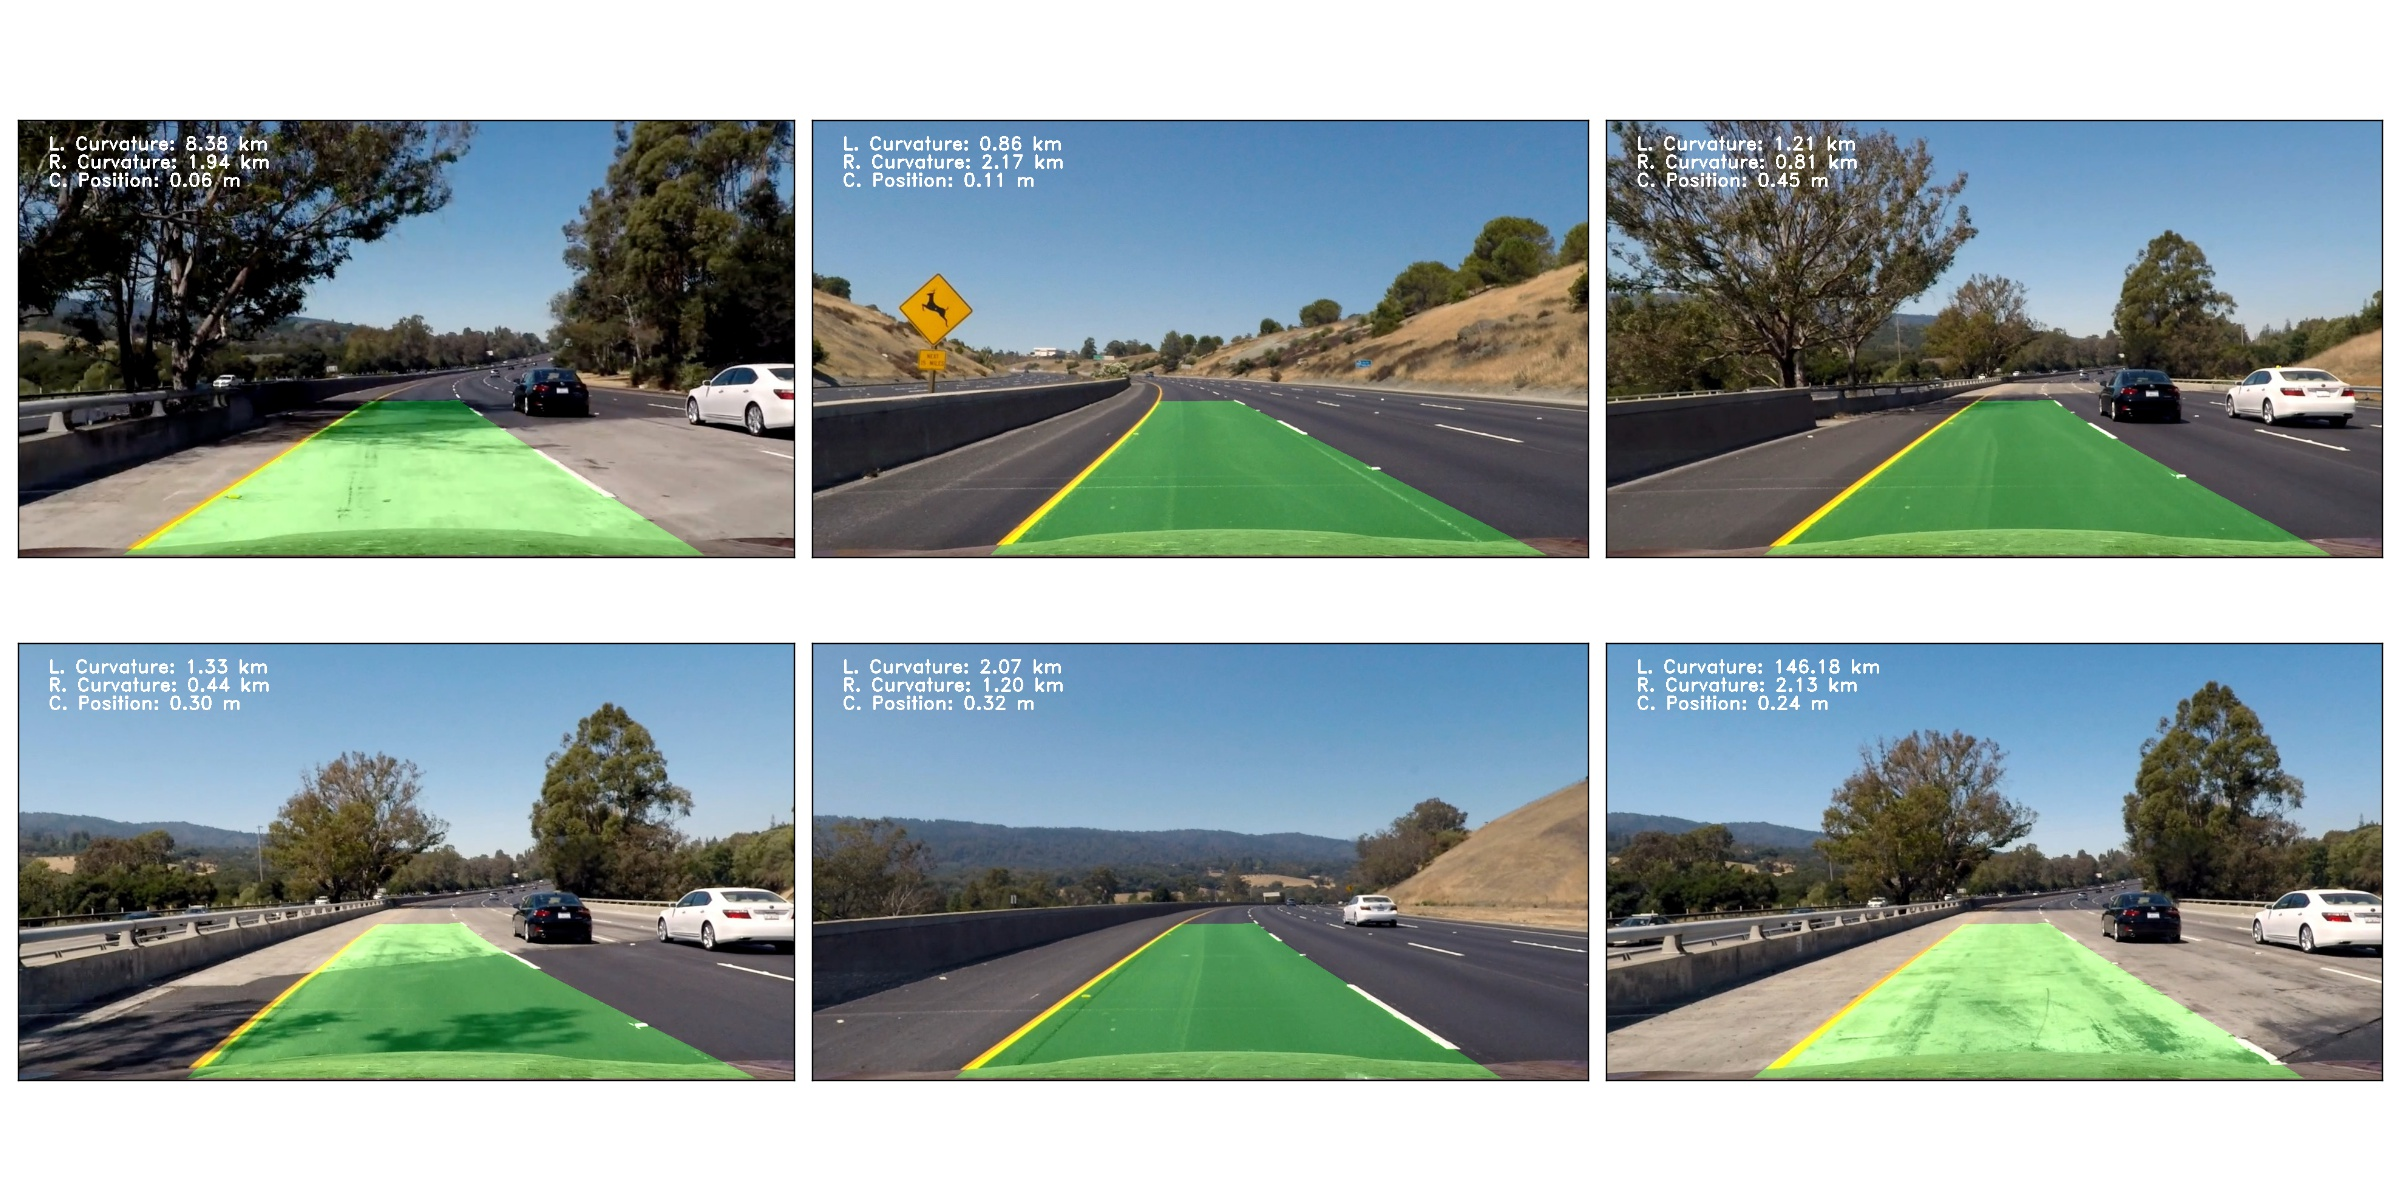
\includegraphics[width=.9\linewidth]{output_images/drawn_lanes_test_images.jpg}

\begin{verbatim}
def get_processor(nbins=10):
    bins = nbins
    l_params = deque(maxlen=bins)
    r_params = deque(maxlen=bins)
    l_radius = deque(maxlen=bins)
    r_radius = deque(maxlen=bins)
    weights = np.arange(1,bins+1)/bins
    def process_image(img0):
	undistorted = undistort(img0)
	warped_binary = warp(highlight(undistorted))
	l_fit, r_fit, l_res, r_res, l_curverad, r_curverad, _ = detect_lines_sliding_window(warped_binary) if len(l_params)==0 else detect_lines(warped_binary,np.average(l_params,0,weights[-len(l_params):]), np.average(r_params,0,weights[-len(l_params):]))
	l_params.append(l_fit)
	r_params.append(r_fit)
	l_radius.append(l_curverad)
	r_radius.append(r_curverad)
	annotated_image = draw_lane(undistorted,
				    warped_binary,
				    np.average(l_params,0,weights[-len(l_params):]),
				    np.average(r_params,0,weights[-len(l_params):]),
				    np.average(l_radius,0,weights[-len(l_params):]),
				    np.average(r_radius,0,weights[-len(l_params):]),
				    unwarp)
	return annotated_image
    return process_image
\end{verbatim}

\begin{verbatim}
process = get_processor()
in_clip = VideoFileClip("project_video.mp4")
out_clip = in_clip.fl_image(process)
cProfile.run('out_clip.write_videofile("output_images/project_output.mp4", audio=False)', 'restats')
\end{verbatim}

\subsection*{Discussion}
\label{sec-2-4}

\subsubsection*{What Worked Well}
\label{sec-2-4-1}

\subsubsection*{What Could Be Improved}
\label{sec-2-4-2}
% <a href="http://www.gnu.org/software/emacs/">Emacs</a> 24.5.1 (<a href="http://orgmode.org">Org</a> mode 8.2.10)
\end{document}